\documentclass[12pt,a4paper,oneside]{report}
% ---------------------------------------------------------------------------
% B.Tech project report. Replace every \placeholder{...} (college, names,
% roll numbers, guide, HOD, dates) before printing. Check your university's
% prescribed format (margins, spacing, certificate wording) and adjust.
% ---------------------------------------------------------------------------
\usepackage[margin=1in,left=1.25in]{geometry}
\usepackage{setspace}
\usepackage{amsmath,amssymb}
\usepackage{graphicx}
\usepackage{booktabs}
\usepackage{longtable}
\usepackage{array}
\usepackage{multirow}
\usepackage{xcolor}
\usepackage{listings}
\usepackage{tikz}
\usetikzlibrary{positioning,arrows.meta,calc,fit,shapes.geometric}
\usepackage{caption}
\usepackage{titlesec}
\usepackage{fancyhdr}
\usepackage[nottoc]{tocbibind}
\usepackage{cite}
\usepackage[hidelinks]{hyperref}

\graphicspath{{../results/}}
\onehalfspacing
\newcommand{\placeholder}[1]{\textcolor{red}{#1}}

\titleformat{\chapter}[display]{\normalfont\Large\bfseries\centering}{\chaptertitlename\ \thechapter}{10pt}{\LARGE}
\titlespacing*{\chapter}{0pt}{-20pt}{25pt}

\pagestyle{fancy}
\fancyhf{}
\fancyhead[R]{\small\nouppercase{\leftmark}}
\fancyfoot[C]{\thepage}
\renewcommand{\headrulewidth}{0.4pt}
\fancypagestyle{plain}{\fancyhf{}\fancyfoot[C]{\thepage}\renewcommand{\headrulewidth}{0pt}}

\lstdefinelanguage{VerilogX}[]{Verilog}{morekeywords={generate,endgenerate,localparam,genvar}}
\lstset{
  basicstyle=\ttfamily\scriptsize,
  keywordstyle=\color{blue!60!black}\bfseries,
  commentstyle=\color{green!40!black}\itshape,
  stringstyle=\color{red!60!black},
  numbers=left, numberstyle=\tiny\color{gray}, stepnumber=1, numbersep=6pt,
  frame=single, rulecolor=\color{gray!60}, breaklines=true, columns=fullflexible,
  showstringspaces=false, tabsize=4, captionpos=b
}

\begin{document}

% =========================================================== TITLE PAGE
\begin{titlepage}
\centering
{\large \placeholder{A Project Report on}\par}
\vspace{0.8cm}
{\LARGE\bfseries Design and FPGA Implementation of a Significance-Driven Hybrid Approximate 8$\times$8 Multiplier for Error-Tolerant Image Processing\par}
\vspace{1cm}
{\large Submitted in partial fulfilment of the requirements for the award of the degree of\par}
\vspace{0.3cm}
{\Large\bfseries Bachelor of Technology\par}
{\large in\par}
{\Large\bfseries Electronics and Communication Engineering\par}
\vspace{1cm}
{\large by\par}
\vspace{0.3cm}
\begin{tabular}{ll}
\placeholder{Student Name 1} & \placeholder{Roll No. XXXXXXXX} \\
\placeholder{Student Name 2} & \placeholder{Roll No. XXXXXXXX} \\
\placeholder{Student Name 3} & \placeholder{Roll No. XXXXXXXX} \\
\end{tabular}
\vspace{1cm}

{\large Under the guidance of\par}
{\large\bfseries \placeholder{Dr./Prof. Guide Name}\par}
{\placeholder{Designation, Department of ECE}\par}
\vfill
{\large Department of Electronics and Communication Engineering\par}
{\large\bfseries \placeholder{College Name}\par}
{\placeholder{(Affiliated to University Name)}\par}
{\placeholder{City -- PIN, State, India}\par}
\vspace{0.3cm}
{\large \placeholder{Month Year}\par}
\end{titlepage}

\pagenumbering{roman}
\setcounter{page}{2}

% =========================================================== CERTIFICATE
\chapter*{Certificate}
\addcontentsline{toc}{chapter}{Certificate}
This is to certify that the project report entitled \textbf{``Design and FPGA Implementation of a Significance-Driven Hybrid Approximate 8$\times$8 Multiplier for Error-Tolerant Image Processing''} submitted by \placeholder{Student Name 1 (Roll No.)}, \placeholder{Student Name 2 (Roll No.)} and \placeholder{Student Name 3 (Roll No.)} in partial fulfilment of the requirements for the award of the degree of Bachelor of Technology in Electronics and Communication Engineering of \placeholder{University Name} is a record of bona fide work carried out by them under my supervision during the academic year \placeholder{20XX--20XX}.

\vspace{2.5cm}
\noindent
\begin{tabular}{@{}p{0.48\textwidth}p{0.48\textwidth}@{}}
\placeholder{Guide Name} & \placeholder{HOD Name} \\
Project Guide & Head of the Department \\
Department of ECE & Department of ECE \\
\end{tabular}

\vspace{2cm}
\noindent External Examiner \hfill Date: \underline{\hspace{3cm}}

% =========================================================== DECLARATION
\chapter*{Declaration}
\addcontentsline{toc}{chapter}{Declaration}
We hereby declare that the project report entitled \textbf{``Design and FPGA Implementation of a Significance-Driven Hybrid Approximate 8$\times$8 Multiplier for Error-Tolerant Image Processing''} is a record of original work carried out by us under the guidance of \placeholder{Guide Name}, and has not been submitted elsewhere for the award of any degree or diploma. Wherever the work of others has been used, it has been duly acknowledged and referenced. Parts of the Verilog code and of this report were drafted with the assistance of an AI tool; we have reviewed, executed and verified all code and results, and we take full responsibility for the content.

\vspace{2cm}
\noindent Place: \placeholder{City}\\
Date: \placeholder{DD/MM/YYYY}
\hfill
\begin{tabular}{r}
\placeholder{Student Name 1} \\ \placeholder{Student Name 2} \\ \placeholder{Student Name 3}
\end{tabular}

% =========================================================== ACKNOWLEDGEMENT
\chapter*{Acknowledgement}
\addcontentsline{toc}{chapter}{Acknowledgement}
We express our sincere gratitude to our project guide, \placeholder{Guide Name}, for continuous guidance, encouragement and valuable suggestions throughout this work. We thank \placeholder{HOD Name}, Head of the Department of Electronics and Communication Engineering, and \placeholder{Principal Name}, Principal, \placeholder{College Name}, for providing the facilities required for the project. We also thank the faculty and laboratory staff of the department, and our families and friends for their support.

\vspace{1.5cm}
\hfill
\begin{tabular}{r}
\placeholder{Student Name 1} \\ \placeholder{Student Name 2} \\ \placeholder{Student Name 3}
\end{tabular}

% =========================================================== ABSTRACT
\chapter*{Abstract}
\addcontentsline{toc}{chapter}{Abstract}
Multiplication is the most resource-hungry arithmetic operation in digital signal processing, image processing and machine-learning hardware. Many of these applications are \emph{error tolerant}: small numerical errors in individual products do not produce visible or meaningful changes in the final output. Approximate computing exploits this tolerance by deliberately simplifying arithmetic circuits to save hardware.

This project designs, verifies and evaluates a family of six 8$\times$8 unsigned multipliers written in Verilog HDL for FPGA implementation. The multipliers are built recursively from 2$\times$2 blocks. Approximation is applied selectively to the partial products of lowest significance, using either the under-designed 2$\times$2 multiplier of Kulkarni \emph{et al.}\ or complete removal (truncation) of the least-significant 4$\times$4 partial product. The proposed hybrid design (HYB) combines both techniques.

All designs were verified exhaustively over the 65{,}536 possible input pairs with a self-checking testbench in Icarus Verilog, and cross-checked against an independent Python model. Synthesis with Yosys for the Xilinx 7-series (Artix-7) fabric of the Basys-3 board shows that HYB needs 80 LUTs instead of 112 for the exact design, a 28.6\% reduction, with a normalised mean error distance of 0.24\%. In three image-processing applications (image multiplication, Gaussian smoothing and image blending) computed from the RTL outputs, HYB achieves a PSNR of 46.7--50.1\,dB and an SSIM of at least 0.996 compared with exact multiplication. The study also shows that, at the LUT granularity of FPGAs, removing the lowest partial product gives a better accuracy--area trade-off than approximating higher partial products.

\vspace{0.5cm}
\noindent\textbf{Keywords:} approximate computing, approximate multiplier, FPGA, Verilog HDL, Artix-7, Basys-3, image processing, PSNR, SSIM.

% =========================================================== LISTS
\tableofcontents
\listoffigures
\listoftables

\chapter*{List of Abbreviations}
\addcontentsline{toc}{chapter}{List of Abbreviations}
\begin{tabular}{@{}ll@{}}
ASIC & Application-Specific Integrated Circuit \\
CARRY4 & Xilinx 7-series 4-bit carry-chain primitive \\
CLB & Configurable Logic Block \\
DSP & Digital Signal Processing \\
ED & Error Distance \\
ER & Error Rate \\
FPGA & Field-Programmable Gate Array \\
HDL & Hardware Description Language \\
HYB & Proposed hybrid approximate multiplier \\
LUT & Look-Up Table \\
MED & Mean Error Distance \\
MRED & Mean Relative Error Distance \\
NMED & Normalised Mean Error Distance \\
PSNR & Peak Signal-to-Noise Ratio \\
RTL & Register-Transfer Level \\
SSIM & Structural Similarity Index Measure \\
UDM & Under-Designed Multiplier \\
WCE & Worst-Case Error \\
XDC & Xilinx Design Constraints \\
\end{tabular}

\clearpage
\pagenumbering{arabic}

% =========================================================== CHAPTER 1
\chapter{Introduction}

\section{Background}
Digital systems for image processing, audio processing, communications and machine learning perform very large numbers of multiplications. A single 3$\times$3 convolution on a 512$\times$512 image needs more than two million multiply operations, and a small neural network needs millions more. In hardware, the multiplier is usually the largest and most power-hungry arithmetic unit, so its cost dominates the cost of the whole datapath.

Field-Programmable Gate Arrays (FPGAs) are widely used to accelerate such workloads because they can implement many operations in parallel and can be reprogrammed. On an FPGA, logic is built from small look-up tables (LUTs), dedicated carry chains, and a limited number of hard DSP blocks. Low-cost FPGAs used in education and embedded products, such as the Artix-7 XC7A35T on the Digilent Basys-3 board, have only 90 DSP slices~\cite{basys3rm}. Once these are used up, every additional multiplier must be built from LUTs, and LUT-efficient multiplier design becomes important.

\section{Approximate Computing}
Many applications do not need exact results. The human eye cannot see a one-level change in a pixel value; a classifier usually outputs the same label even if its internal products carry small errors; and sensor data already contain noise. \emph{Approximate computing} exploits this error tolerance by simplifying hardware so that it produces slightly inexact results in exchange for lower area, delay or energy~\cite{han2013approximate,mittal2016survey}. Arithmetic circuits, especially adders and multipliers, are the most studied targets~\cite{jiang2020survey}.

\section{Problem Statement}
Most approximate multipliers in the literature were designed and evaluated for ASICs, where savings are counted in gates or transistors. On an FPGA, a design that removes a few gates may not remove any LUT, because a 6-input LUT implements any function of up to six inputs at the same cost. The problem addressed in this project is therefore:

\begin{quote}
\emph{Where, within a recursive 8$\times$8 multiplier, should approximation be applied to obtain the best trade-off between LUT usage and output quality on a low-cost FPGA, and how do such multipliers perform in real image-processing tasks?}
\end{quote}

\section{Objectives}
\begin{enumerate}
\item Design an exact recursive 8$\times$8 unsigned multiplier in Verilog HDL from 2$\times$2 building blocks.
\item Design approximate variants that apply approximation at different significance levels, using the under-designed 2$\times$2 multiplier and partial-product truncation, and propose a hybrid design.
\item Verify every design exhaustively with a self-checking testbench and produce simulation waveforms.
\item Characterise the error of every design using standard metrics (ER, MED, NMED, MRED, WCE).
\item Synthesise every design for the Xilinx 7-series (Artix-7) fabric and compare LUT, carry-chain and logic-depth figures.
\item Evaluate the multipliers in image multiplication, Gaussian smoothing and image blending using PSNR and SSIM.
\item Build a Basys-3 demonstration that lets a user select the multiplier and see the product and error on the board.
\end{enumerate}

\section{Methodology Overview}
Figure~\ref{fig:flow} summarises the design flow. The RTL is written in Verilog, simulated with Icarus Verilog, synthesised with Yosys for the Xilinx 7-series fabric, and analysed with Python. All steps are scripted, so every number in this report can be regenerated with one command (\texttt{run\_all.sh}).

\begin{figure}[ht]
\centering
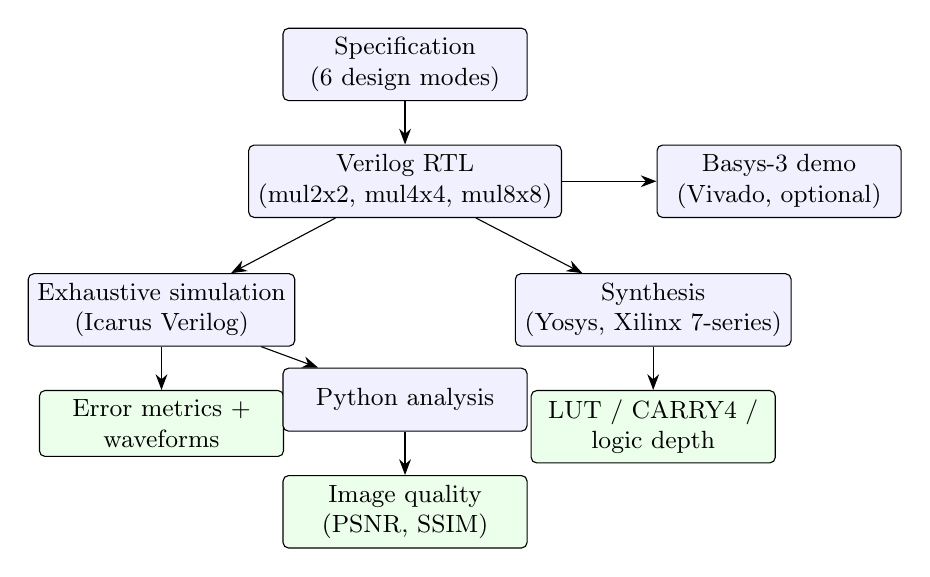
\begin{tikzpicture}[node distance=0.55cm and 0.6cm,
  box/.style={draw, rounded corners=2pt, fill=blue!6, minimum width=3.1cm, minimum height=0.8cm, align=center, font=\small},
  resbox/.style={draw, rounded corners=2pt, fill=green!8, minimum width=3.1cm, minimum height=0.8cm, align=center, font=\small},
  >={Stealth[length=2mm]}]
\node[box] (spec) {Specification\\(6 design modes)};
\node[box, below=of spec] (rtl) {Verilog RTL\\(mul2x2, mul4x4, mul8x8)};
\node[box, below left=0.7cm and -0.6cm of rtl] (sim) {Exhaustive simulation\\(Icarus Verilog)};
\node[box, below right=0.7cm and -0.6cm of rtl] (syn) {Synthesis\\(Yosys, Xilinx 7-series)};
\node[resbox, below=of sim] (err) {Error metrics +\\waveforms};
\node[resbox, below=of syn] (res) {LUT / CARRY4 /\\logic depth};
\node[box, below=1.9cm of rtl] (py) {Python analysis};
\node[resbox, below=of py] (img) {Image quality\\(PSNR, SSIM)};
\node[box, right=1.2cm of rtl] (fpga) {Basys-3 demo\\(Vivado, optional)};
\draw[->] (spec) -- (rtl);
\draw[->] (rtl) -- (sim);
\draw[->] (rtl) -- (syn);
\draw[->] (rtl) -- (fpga);
\draw[->] (sim) -- (err);
\draw[->] (syn) -- (res);
\draw[->] (sim) -- (py);
\draw[->] (py) -- (img);
\end{tikzpicture}
\caption{Design and evaluation flow used in this project.}
\label{fig:flow}
\end{figure}

\section{Organisation of the Report}
Chapter~2 reviews the literature on approximate computing and approximate multipliers. Chapter~3 presents the theory of binary multiplication, recursive decomposition, FPGA architecture and quality metrics. Chapter~4 describes the proposed multiplier family and its Verilog implementation. Chapter~5 explains the verification, synthesis and application methodology. Chapter~6 presents and discusses the results. Chapter~7 concludes the report and outlines future work. The appendices contain the complete source code and instructions to reproduce the results.

% =========================================================== CHAPTER 2
\chapter{Literature Survey}

\section{Approximate Computing}
Han and Orshansky~\cite{han2013approximate} described approximate computing as an emerging paradigm for energy-efficient design, in which the requirement for exact computation is relaxed for applications that can tolerate errors. Mittal's survey~\cite{mittal2016survey} classifies approximation techniques at the circuit, architecture and software levels, and identifies image processing, multimedia and machine learning as the main beneficiaries. At the circuit level, approximate adders and multipliers are the most common building blocks.

\section{Approximate Arithmetic Circuits}
Jiang \emph{et al.}~\cite{jiang2020survey} survey and characterise a large number of approximate adders, multipliers and dividers. They define the error metrics used in this report (error rate, mean error distance, normalised and relative error distances) and show that the best design depends strongly on the application and on the implementation technology. Approximate multipliers are generally built by (i) approximating the partial-product generation, (ii) approximating the partial-product accumulation, or (iii) truncating low-order bits or partial products.

\section{Under-Designed Multiplier}
Kulkarni, Gupta and Ercegovac~\cite{kulkarni2011udm} proposed an under-designed 2$\times$2 multiplier block that is exact for 15 of its 16 input combinations; for $3\times3$ it outputs 7 instead of 9. Because the output then fits in three bits, the block is smaller, and larger multipliers built from it recursively inherit the saving. The resulting error is always an under-estimate. This block is the basis of three of the designs in this project.

\section{Architectural Exploration of Approximate Multipliers}
Rehman \emph{et al.}~\cite{rehman2016space} explored the architectural space of approximate multipliers built from approximate elementary blocks and approximate adders, showing that the placement of approximate blocks has a large effect on the accuracy--cost trade-off. This project applies a similar placement idea, but targets FPGA LUT cost and adds partial-product truncation as a second technique.

\section{FPGA-Specific Approximate Multipliers}
Ullah \emph{et al.}~\cite{ullah2022fpga} showed that multipliers designed for ASICs do not necessarily give the same savings on FPGAs, and proposed accurate and approximate multipliers that exploit the LUT and carry-chain structure of Xilinx FPGAs. Vakili \emph{et al.}\ proposed DyRecMul~\cite{vakili2024dyrecmul}, which uses dynamically reconfigurable LUT primitives; they report LUT reductions of 64\% for signed 8-bit multiplication compared with the standard Xilinx multiplier core, with an average accuracy loss below 0.29\% on deep-learning benchmarks. Kida and Sato~\cite{kida2025fourbit} showed that a carefully hand-structured exact 4-bit multiplier on 7-series FPGAs needs only 11 LUTs and two CARRY4 blocks, and that Vivado does not infer this structure from a behavioural \texttt{a*b}.

\section{Summary and Research Gap}
Table~\ref{tab:lit} summarises the reviewed work. Existing FPGA-oriented approximate multipliers achieve large savings but often rely on device-specific primitives, dynamic reconfiguration or hand-placed LUT initialisation, which makes them hard to reproduce in a student project. There is room for a simple, fully portable study that uses only standard Verilog, open-source tools and a low-cost board, and that answers where approximation should be placed within a recursive multiplier to minimise LUT usage for a given error.

\begin{table}[ht]
\centering
\caption{Summary of related work}
\label{tab:lit}
\small
\begin{tabular}{p{3.2cm}p{4.3cm}p{5.8cm}}
\toprule
Work & Technique & Relevance to this project \\
\midrule
Han \& Orshansky~\cite{han2013approximate} & Approximate computing paradigm & Motivation for trading accuracy for cost \\
Mittal~\cite{mittal2016survey} & Survey of techniques & Application domains, levels of approximation \\
Jiang \emph{et al.}~\cite{jiang2020survey} & Survey of approximate arithmetic & Error metrics used in Chapter~6 \\
Kulkarni \emph{et al.}~\cite{kulkarni2011udm} & Under-designed 2$\times$2 block & Approximate building block \\
Rehman \emph{et al.}~\cite{rehman2016space} & Architectural space exploration & Placement of approximate blocks \\
Ullah \emph{et al.}~\cite{ullah2022fpga} & FPGA-specific multipliers & FPGA cost differs from ASIC cost \\
Vakili \emph{et al.}~\cite{vakili2024dyrecmul} & Dynamic LUT reconfiguration & State-of-the-art LUT savings \\
Kida \& Sato~\cite{kida2025fourbit} & Hand-structured 4-bit multiplier & Structure matters on 7-series LUTs \\
\bottomrule
\end{tabular}
\end{table}

% =========================================================== CHAPTER 3
\chapter{Theoretical Background}

\section{Binary Multiplication}
For unsigned $n$-bit operands $A=\sum_{i=0}^{n-1}a_i2^i$ and $B=\sum_{j=0}^{n-1}b_j2^j$, the product is
\begin{equation}
P = AB = \sum_{i=0}^{n-1}\sum_{j=0}^{n-1} a_ib_j\,2^{i+j}.
\end{equation}
Each term $a_ib_j$ is a partial-product bit produced by an AND gate. An array multiplier adds these $n^2$ bits with rows of adders. The product of two 8-bit numbers needs 16 bits, and the largest product is $255\times255=65{,}025$.

\section{Recursive (Divide-and-Conquer) Multiplication}
Splitting each operand into a high half and a low half, $A=2^{n/2}A_H+A_L$ and $B=2^{n/2}B_H+B_L$, gives
\begin{equation}
AB = 2^{n}A_HB_H + 2^{n/2}(A_HB_L + A_LB_H) + A_LB_L .
\label{eq:rec}
\end{equation}
An 8$\times$8 multiplier therefore needs four 4$\times$4 multipliers and an adder, and each 4$\times$4 multiplier needs four 2$\times$2 multipliers. Equation~\eqref{eq:rec} makes the \emph{significance} of each partial product explicit: an error in $A_LB_L$ is multiplied by $2^0$, an error in $A_HB_L$ or $A_LB_H$ by $2^4$, and an error in $A_HB_H$ by $2^8$.

\section{Exact and Approximate 2$\times$2 Multipliers}
Table~\ref{tab:tt} gives the truth table of the exact and approximate 2$\times$2 multipliers. The exact block needs four output bits:
\begin{align}
p_0 &= a_0b_0, & p_1 &= a_1b_0 \oplus a_0b_1,\\
p_2 &= a_1b_1 \oplus a_1a_0b_1b_0, & p_3 &= a_1a_0b_1b_0 .
\end{align}
The under-designed block of Kulkarni \emph{et al.}~\cite{kulkarni2011udm} replaces the XOR in $p_1$ with an OR and drops $p_3$:
\begin{equation}
p_0 = a_0b_0,\qquad p_1 = a_1b_0 \lor a_0b_1,\qquad p_2 = a_1b_1,\qquad p_3 = 0 .
\end{equation}
It differs from the exact block only for $A=B=3$, where it returns $7$ instead of $9$ (an error of 2, i.e.\ 22\%).

\begin{table}[ht]
\centering
\caption{Truth table of the exact and approximate 2$\times$2 multipliers (products in decimal)}
\label{tab:tt}
\begin{tabular}{cccc|cccc}
\toprule
$A$ & $B$ & Exact & Approx & $A$ & $B$ & Exact & Approx \\
\midrule
0 & 0 & 0 & 0 & 2 & 0 & 0 & 0 \\
0 & 1 & 0 & 0 & 2 & 1 & 2 & 2 \\
0 & 2 & 0 & 0 & 2 & 2 & 4 & 4 \\
0 & 3 & 0 & 0 & 2 & 3 & 6 & 6 \\
1 & 0 & 0 & 0 & 3 & 0 & 0 & 0 \\
1 & 1 & 1 & 1 & 3 & 1 & 3 & 3 \\
1 & 2 & 2 & 2 & 3 & 2 & 6 & 6 \\
1 & 3 & 3 & 3 & 3 & 3 & \textbf{9} & \textbf{7} \\
\bottomrule
\end{tabular}
\end{table}

\section{Partial-Product Truncation}
Truncation removes a partial product completely. Removing $A_LB_L$ from~\eqref{eq:rec} saves one 4$\times$4 multiplier and one adder input. The maximum error is the largest value of $A_LB_L$, $15\times15=225$, which is 0.35\% of the full-scale product. The error rate, however, is high, because $A_LB_L$ is non-zero for most inputs.

\section{FPGA Architecture}
\subsection{Look-up tables and carry chains}
Xilinx 7-series FPGAs are built from configurable logic blocks (CLBs), each containing two slices~\cite{ug474}. Each slice has four 6-input LUTs, eight flip-flops, wide-function multiplexers (MUXF7, MUXF8) and a 4-bit carry chain (CARRY4). A 6-input LUT can implement \emph{any} Boolean function of up to six inputs, so the cost of a function depends on how many LUTs its outputs require, not on how many gates it contains.

\subsection{Basys-3 board}
The Digilent Basys-3 board~\cite{basys3rm} carries an Artix-7 XC7A35T-1CPG236C FPGA with 33{,}280 logic cells in 5{,}200 slices, 1{,}800\,Kbit of block RAM and 90 DSP slices, together with 16 switches, 16 LEDs, five push-buttons, a four-digit seven-segment display and a 100\,MHz oscillator. Designs are developed with the free Vivado WebPACK edition.

\section{Error Metrics}
Let $P$ be the exact product, $\tilde{P}$ the approximate product, $ED=|P-\tilde{P}|$ the error distance, and $P_{\max}=255^2$. Over all $N=65{,}536$ input pairs~\cite{jiang2020survey}:
\begin{align}
\text{ER} &= \frac{\#\{ED>0\}}{N}\times100\%, &
\text{MED} &= \frac{1}{N}\sum ED, \\
\text{NMED} &= \frac{\text{MED}}{P_{\max}}\times100\%, &
\text{MRED} &= \frac{1}{N'}\sum_{P\neq0}\frac{ED}{P}\times100\%, \\
\text{WCE} &= \max ED . &&
\end{align}
where $N'$ is the number of input pairs with non-zero exact product.

\section{Image Quality Metrics}
For an $M\times N$ 8-bit image $I$ and its approximate version $\tilde{I}$, the mean squared error and peak signal-to-noise ratio are
\begin{equation}
\text{MSE}=\frac{1}{MN}\sum_{x,y}\bigl(I(x,y)-\tilde{I}(x,y)\bigr)^2,\qquad
\text{PSNR}=10\log_{10}\frac{255^2}{\text{MSE}}\ \text{dB}.
\end{equation}
The structural similarity index (SSIM)~\cite{wang2004ssim} compares local luminance, contrast and structure and ranges from 0 to 1, where 1 means identical images. PSNR above about 40\,dB and SSIM above 0.99 are generally considered visually lossless.

% =========================================================== CHAPTER 4
\chapter{Proposed Design}

\section{Design Space}
The 8$\times$8 multiplier is built according to~\eqref{eq:rec}. For each of the four 4$\times$4 partial products the designer can choose one of three options: exact (built from exact 2$\times$2 blocks), approximate (built from under-designed 2$\times$2 blocks), or removed (truncated). Following the significance of each term, approximation is introduced from the least-significant partial product upwards. Table~\ref{tab:modes} lists the six configurations implemented, and Figure~\ref{fig:arch} shows the proposed hybrid.

\begin{table}[ht]
\centering
\caption{Multiplier configurations (MODE parameter of \texttt{mul8x8})}
\label{tab:modes}
\begin{tabular}{clcccc}
\toprule
MODE & Name & $A_LB_L$ ($2^0$) & $A_HB_L$ ($2^4$) & $A_LB_H$ ($2^4$) & $A_HB_H$ ($2^8$) \\
\midrule
0 & EXACT   & exact  & exact  & exact  & exact \\
1 & AM-L    & approx & exact  & exact  & exact \\
2 & AM-LM   & approx & approx & approx & exact \\
3 & AM-ALL  & approx & approx & approx & approx \\
4 & TRUNC-L & removed & exact & exact  & exact \\
5 & \textbf{HYB} & removed & approx & approx & exact \\
\bottomrule
\end{tabular}
\end{table}

\begin{figure}[ht]
\centering
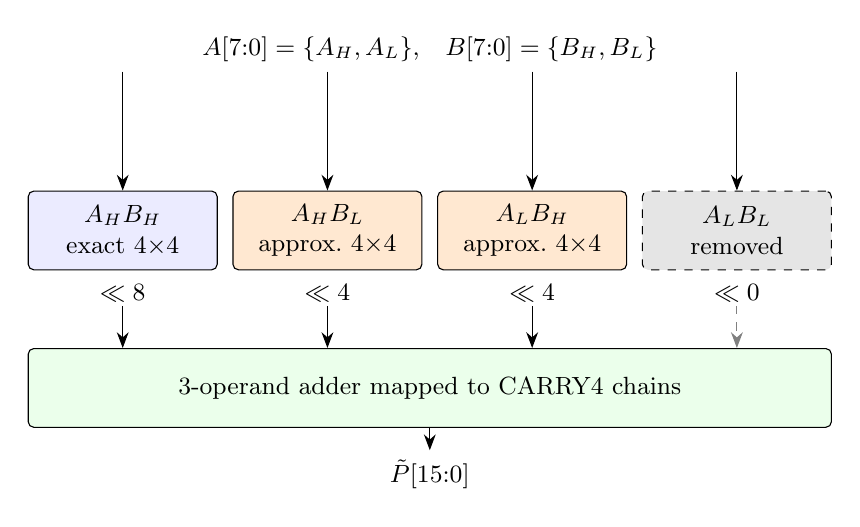
\begin{tikzpicture}[
  blk/.style={draw, rounded corners=2pt, minimum width=2.4cm, minimum height=1cm, font=\small, align=center},
  ex/.style={blk, fill=blue!8},
  ap/.style={blk, fill=orange!18},
  tr/.style={blk, fill=gray!20, dashed},
  >={Stealth[length=2mm]}]
\node[font=\small] (A) at (3.9,2.3) {$A[7{:}0]=\{A_H,A_L\}$,\quad $B[7{:}0]=\{B_H,B_L\}$};
\node[ex] (hh) at (0,0)    {$A_HB_H$\\exact 4$\times$4};
\node[ap] (hl) at (2.6,0)  {$A_HB_L$\\approx.\ 4$\times$4};
\node[ap] (lh) at (5.2,0)  {$A_LB_H$\\approx.\ 4$\times$4};
\node[tr] (ll) at (7.8,0)  {$A_LB_L$\\removed};
\foreach \n in {hh,hl,lh,ll} \draw[->] (A.south -| \n.north) -- (\n.north);
\node[font=\small] at (0,-0.8)   {$\ll 8$};
\node[font=\small] at (2.6,-0.8) {$\ll 4$};
\node[font=\small] at (5.2,-0.8) {$\ll 4$};
\node[font=\small] at (7.8,-0.8) {$\ll 0$};
\node[blk, minimum width=10.2cm, fill=green!8] (add) at (3.9,-2) {3-operand adder mapped to CARRY4 chains};
\foreach \n in {hh,hl,lh} \draw[->] (\n.south) ++(0,-0.45) -- (\n.south |- add.north);
\draw[->, dashed, gray] (ll.south) ++(0,-0.45) -- (ll.south |- add.north);
\node[font=\small] (P) at (3.9,-3.1) {$\tilde{P}[15{:}0]$};
\draw[->] (add) -- (P);
\end{tikzpicture}
\caption{Architecture of the proposed hybrid (HYB) 8$\times$8 multiplier. Each approximate 4$\times$4 block is built from four under-designed 2$\times$2 blocks.}
\label{fig:arch}
\end{figure}

\section{Properties of the Design Family}
\begin{itemize}
\item \textbf{One-sided error.} Both the under-designed block and truncation can only reduce a partial product, so every approximate design satisfies $\tilde{P}\le P$. The error is always an under-estimate, which simplifies analysis and allows constant compensation.
\item \textbf{Exact high-order term.} Except in AM-ALL, the most significant partial product $A_HB_H$ is exact, which bounds the error for large operands.
\item \textbf{Bounded error for truncation.} TRUNC-L can never be wrong by more than 225.
\item \textbf{Zero output for small operands.} TRUNC-L and HYB return zero whenever both operands are below 16, because the whole product lies in the removed $A_LB_L$ term. These designs therefore suit data dominated by mid-to-high values, such as natural images.
\end{itemize}

\section{Verilog Implementation}
\subsection{2$\times$2 blocks}
Listing~\ref{lst:m2} shows the exact and approximate 2$\times$2 blocks written directly from the Boolean equations of Section~3.3.

\lstinputlisting[language=VerilogX, caption={2$\times$2 multiplier blocks (\texttt{rtl/mul2x2.v})}, label=lst:m2]{../rtl/mul2x2.v}

\subsection{4$\times$4 block}
The 4$\times$4 module instantiates four 2$\times$2 blocks inside a \texttt{generate} statement selected by the \texttt{APPROX} parameter, and combines them with shifts and additions (Listing~\ref{lst:m4}).

\lstinputlisting[language=VerilogX, caption={Recursive 4$\times$4 multiplier (\texttt{rtl/mul4x4.v})}, label=lst:m4]{../rtl/mul4x4.v}

\subsection{8$\times$8 multiplier}
The 8$\times$8 module (Listing~\ref{lst:m8}) derives the configuration of each 4$\times$4 block from the \texttt{MODE} parameter with \texttt{localparam} expressions, so a single module describes all six designs. The file also contains the behavioural reference \texttt{mul8x8\_beh}.

\lstinputlisting[language=VerilogX, caption={Parameterised 8$\times$8 multiplier (\texttt{rtl/mul8x8.v})}, label=lst:m8]{../rtl/mul8x8.v}

\subsection{Registered wrapper}
For clocked operation, \texttt{mul8x8\_pipe} registers the inputs and the output, giving a latency of two clock cycles (Appendix~\ref{app:rtl}).

\section{Basys-3 Demonstration System}
The top-level module \texttt{basys3\_top} (Appendix~\ref{app:fpga}) instantiates all six multipliers and lets the user compare them on the board. Table~\ref{tab:io} gives the user interface. Push-buttons are synchronised and sampled every $2^{20}$ clock cycles (about 10\,ms) to remove contact bounce. The seven-segment display is multiplexed across its four digits.

\begin{table}[ht]
\centering
\caption{Basys-3 user interface}
\label{tab:io}
\begin{tabular}{lll}
\toprule
Board resource & Signal & Function \\
\midrule
SW15--SW8 & \texttt{a[7:0]} & Operand $A$ \\
SW7--SW0  & \texttt{b[7:0]} & Operand $B$ \\
LD15--LD0 & \texttt{led[15:0]} & Product of the selected multiplier (binary) \\
BTNU / BTND & \texttt{btnU}, \texttt{btnD} & Next / previous multiplier mode (0--5) \\
BTNC & \texttt{btnC} & Reset (mode 0) \\
7-segment digit 3 & -- & Current mode number \\
7-segment digits 2--0 & -- & Error $P-\tilde{P}$ in hexadecimal (low 12 bits) \\
\bottomrule
\end{tabular}
\end{table}

% =========================================================== CHAPTER 5
\chapter{Implementation and Verification Methodology}

\section{Tools}
\begin{itemize}
\item \textbf{Icarus Verilog}~\cite{iverilog} (version 12) for RTL simulation and VCD waveform generation.
\item \textbf{Yosys}~\cite{yosys} (version 0.33) for synthesis to Xilinx 7-series primitives using the \texttt{synth\_xilinx} command with \texttt{-family xc7}.
\item \textbf{Python 3} with NumPy, Matplotlib and scikit-image~\cite{vanderwalt2014skimage} for error analysis, image processing and plotting.
\item \textbf{Xilinx Vivado} (optional) for place-and-route, timing, power and bitstream generation for the Basys-3 board, using the script in Appendix~\ref{app:fpga}.
\end{itemize}

\section{Exhaustive Functional Verification}
Because each operand has only 256 values, all $2^{16}=65{,}536$ input pairs can be simulated. The testbench \texttt{tb\_exhaustive} (Appendix~\ref{app:tb}) instantiates the behavioural reference and all six designs, applies every input pair, and checks that:
\begin{enumerate}
\item the behavioural and recursive exact multipliers both equal $a\times b$;
\item no approximate design produces a product larger than $a\times b$.
\end{enumerate}
It prints \texttt{RESULT: PASS} only if both checks hold for all inputs, and it writes every product to a text file for analysis. As an independent check, the Python analysis script contains a separate bit-accurate model of each design and confirms that it reproduces the RTL output for all 65{,}536 pairs.

\section{Waveform Simulation}
The clocked testbench \texttt{tb\_wave} drives the registered wrappers of all six designs with a 100\,MHz clock and a sequence of ten operand pairs that includes small values, the $3\times3$ corner case and the maximum $255\times255$. It writes a VCD file, which the analysis script renders as a timing diagram.

\section{Synthesis Methodology}
Every design was synthesised for the Xilinx 7-series fabric with DSP inference disabled (\texttt{-nodsp}), so that all designs are compared on LUTs and carry chains. Two flows were used:
\begin{itemize}
\item \textbf{Hierarchical (primary).} Each module is technology-mapped separately and the netlist is flattened only for counting. The LUT count therefore reflects the structural design.
\item \textbf{Flattened with ABC9 (sensitivity check).} The whole design is flattened before optimisation, allowing the tool to re-optimise across block boundaries.
\end{itemize}
Logic depth is the longest topological path through mapped cells (LUTs and CARRY4), excluding the input and output buffers, and serves as a technology-independent proxy for delay.

\section{Image-Processing Applications}
Three kernels were implemented in Python, with every multiplication looked up from the RTL product tables:
\begin{enumerate}
\item \textbf{Image multiplication:} $O=(I_1\cdot I_2)\gg 8$ for the \emph{camera} and \emph{moon} test images ($512\times512$).
\item \textbf{Gaussian smoothing:} 3$\times$3 kernel with integer weights $\begin{bmatrix}20&32&20\\32&48&32\\20&32&20\end{bmatrix}$ (sum 256) applied to \emph{camera}~\cite{gonzalez2018dip}.
\item \textbf{Image blending:} $O=(\alpha I_1 + (255-\alpha) I_2)\gg 8$ with $\alpha=179$ (about 0.7), blending \emph{camera} and \emph{coins}.
\end{enumerate}
Each approximate output is compared with the exact output using PSNR and SSIM.

% =========================================================== CHAPTER 6
\chapter{Results and Discussion}

\section{Functional Verification}
The exhaustive testbench produced the following output:
\begin{lstlisting}[language={}, numbers=none, caption={Exhaustive testbench console output}]
Vectors applied            : 65536
Exact-design mismatches    : 0
Approx over-estimations    : 0
RESULT: PASS
\end{lstlisting}
Both exact designs are therefore correct for every input, and every approximate design under-estimates or equals the exact product. The Python model matched the RTL output for all designs.

\section{Simulation Waveforms}
Figure~\ref{fig:wave} shows the clocked simulation. Each product appears two clock cycles after its operands because of the input and output registers. Table~\ref{tab:wave} lists the values.

\begin{figure}[ht]
\centering
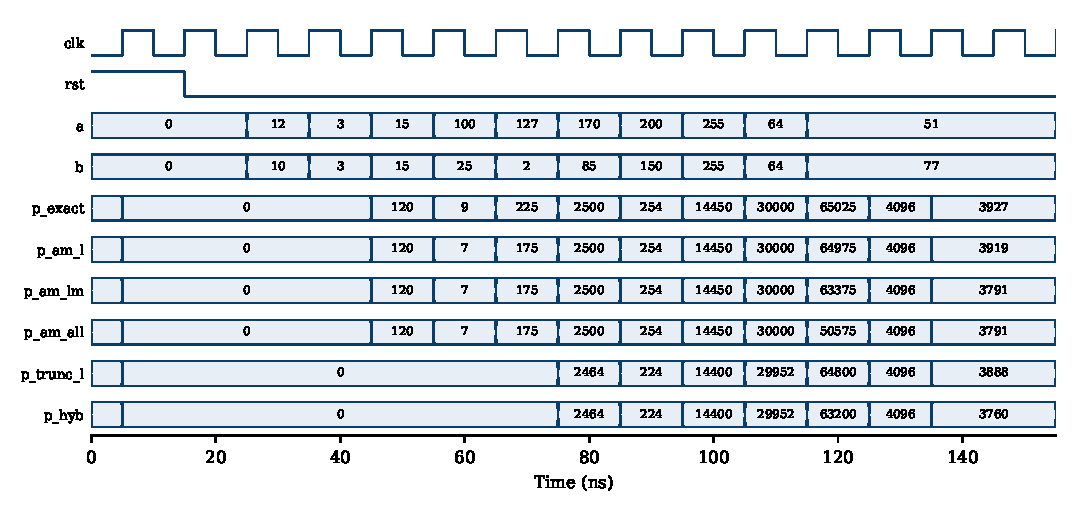
\includegraphics[width=\textwidth]{fig_waveform.pdf}
\caption{Simulation waveform of the six registered multipliers (Icarus Verilog, 100\,MHz clock).}
\label{fig:wave}
\end{figure}

\begin{table}[ht]
\centering
\caption{Products observed in the waveform simulation}
\label{tab:wave}
\small
\begin{tabular}{rrrrrrrr}
\toprule
$A$ & $B$ & EXACT & AM-L & AM-LM & AM-ALL & TRUNC-L & HYB \\
\midrule
12 & 10 & 120 & 120 & 120 & 120 & 0 & 0 \\
3 & 3 & 9 & 7 & 7 & 7 & 0 & 0 \\
15 & 15 & 225 & 175 & 175 & 175 & 0 & 0 \\
100 & 25 & 2500 & 2500 & 2500 & 2500 & 2464 & 2464 \\
127 & 2 & 254 & 254 & 254 & 254 & 224 & 224 \\
170 & 85 & 14450 & 14450 & 14450 & 14450 & 14400 & 14400 \\
200 & 150 & 30000 & 30000 & 30000 & 30000 & 29952 & 29952 \\
255 & 255 & 65025 & 64975 & 63375 & 50575 & 64800 & 63200 \\
64 & 64 & 4096 & 4096 & 4096 & 4096 & 4096 & 4096 \\
51 & 77 & 3927 & 3919 & 3791 & 3791 & 3888 & 3760 \\
\bottomrule
\end{tabular}
\end{table}

The $3\times3$ case shows the under-designed block returning 7. TRUNC-L and HYB return 0 for the first three pairs, whose upper nibbles are all zero, as predicted in Section~4.2. For $64\times64$ every design is exact, because all low-order fields are zero.

\section{Error Characteristics}
Table~\ref{tab:err} summarises the error metrics over all 65{,}536 input pairs, and Figures~\ref{fig:hist} and~\ref{fig:map} show the distribution of the errors.

\begin{table}[ht]
\centering
\caption{Error metrics over all 65{,}536 input pairs}
\label{tab:err}
\begin{tabular}{lrrrrrr}
\toprule
Design & ER (\%) & MED & NMED (\%) & MRED (\%) & WCE & WCE (\%) \\
\midrule
EXACT   & 0.00  & 0.00   & 0.0000 & 0.000 & 0     & 0.00 \\
AM-L    & 19.14 & 3.12   & 0.0048 & 0.076 & 50    & 0.08 \\
AM-LM   & 40.67 & 103.12 & 0.1586 & 0.925 & 1650  & 2.54 \\
AM-ALL  & 46.73 & 903.12 & 1.3889 & 3.280 & 14450 & 22.22 \\
TRUNC-L & 87.89 & 56.25  & 0.0865 & 1.859 & 225   & 0.35 \\
\textbf{HYB} & 90.28 & 156.25 & 0.2403 & 2.708 & 1825 & 2.81 \\
\bottomrule
\end{tabular}
\end{table}

\begin{figure}[ht]
\centering
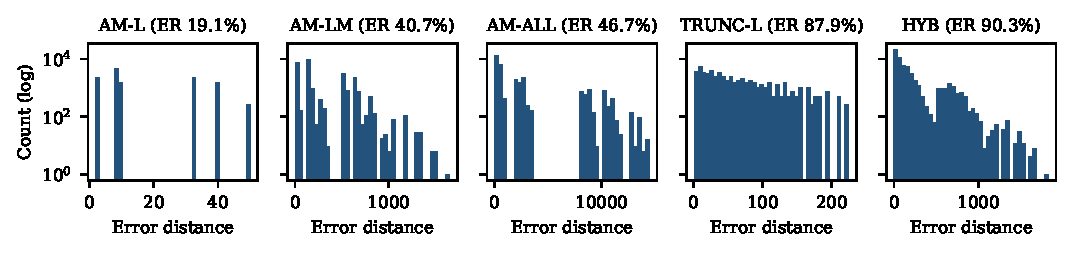
\includegraphics[width=\textwidth]{fig_error_hist.pdf}
\caption{Histograms of non-zero error distances (logarithmic count axis).}
\label{fig:hist}
\end{figure}

\begin{figure}[ht]
\centering
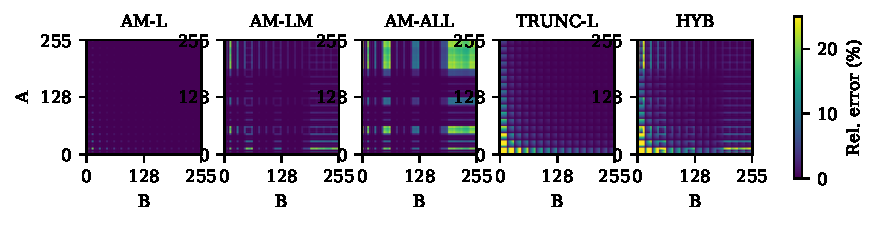
\includegraphics[width=\textwidth]{fig_error_map.pdf}
\caption{Relative error over the operand space ($A$ vertical, $B$ horizontal; colour scale clipped at 25\%).}
\label{fig:map}
\end{figure}

Several observations follow:
\begin{itemize}
\item AM-L is extremely accurate (NMED 0.0048\%, WCE 50), because its only errors are in the lowest-weight partial product.
\item Extending the under-designed block to the middle partial products (AM-LM) raises NMED by a factor of 33, and extending it to $A_HB_H$ (AM-ALL) raises the worst-case error to 22\% of full scale.
\item TRUNC-L is wrong for 88\% of inputs, but its errors are small and bounded (WCE 225, NMED 0.0865\%), so it is more accurate on average than AM-LM.
\item HYB combines the two: NMED 0.24\% and WCE 1825 (2.8\% of full scale).
\item For TRUNC-L and HYB, the largest relative errors appear at small operands, while AM-ALL also has large relative errors at large operands (Figure~\ref{fig:map}).
\end{itemize}

\section{FPGA Resource Utilisation}
Table~\ref{tab:syn} gives the synthesis results for the Xilinx 7-series fabric.

\begin{table}[ht]
\centering
\caption{Synthesis results for the Xilinx 7-series fabric (Yosys, DSP inference disabled)}
\label{tab:syn}
\begin{tabular}{lrrrrrr}
\toprule
 & \multicolumn{5}{c}{Hierarchical flow (primary)} & Flat ABC9 \\
\cmidrule(lr){2-6}
Design & LUT & LUT6 & CARRY4 & Depth & Saving & LUT \\
\midrule
Behavioural \texttt{a*b} & 113$^\dagger$ & 76 & 4 & 9 & $-0.9$\% & 103 \\
EXACT   & 112 & 19 & 12 & 8 & --     & 103 \\
AM-L    & 108 & 19 & 12 & 8 & 3.6\%  & 120 \\
AM-LM   & 100 & 19 & 12 & 8 & 10.7\% & 97 \\
AM-ALL  & 96  & 19 & 12 & 8 & 14.3\% & 88 \\
TRUNC-L & 88  & 12 & 10 & 7 & 21.4\% & 82 \\
\textbf{HYB} & \textbf{80} & 12 & 10 & 7 & \textbf{28.6\%} & \textbf{62} \\
\bottomrule
\multicolumn{7}{l}{\footnotesize $^\dagger$ plus 22 MUXF7 and 1 MUXF8 cells; with DSP inference allowed it maps to one DSP48E1.}
\end{tabular}
\end{table}

\subsection{Discussion}
\begin{itemize}
\item The exact recursive design uses 112 LUTs, almost identical to the behavioural \texttt{a*b} (113 LUTs plus 23 wide multiplexers). The recursive structure therefore costs nothing in the hierarchical flow.
\item Each under-designed 2$\times$2 block saves exactly one LUT, because its fourth output is the constant 0. AM-L, AM-LM and AM-ALL replace 4, 12 and 16 blocks and save 4, 12 and 16 LUTs respectively.
\item Truncation removes a whole 4$\times$4 block and one adder operand, saving 24 LUTs and two CARRY4 cells and shortening the logic depth from 8 to 7.
\item HYB saves 32 LUTs (28.6\%), the largest reduction among the designs.
\item In the flattened flow the tool re-optimises across blocks. It confirms the large savings (HYB: 62 versus 103 LUTs, a 39.8\% reduction), but AM-L becomes larger than EXACT (120 versus 103). Small approximations are therefore sensitive to synthesis heuristics, while the savings of truncation and HYB are robust.
\end{itemize}

\section{Accuracy--Area Trade-off}
Figure~\ref{fig:trade} plots LUT count against NMED. A design is \emph{Pareto-optimal} if no other design is both smaller and more accurate. EXACT, AM-L, TRUNC-L and HYB are Pareto-optimal; AM-LM and AM-ALL are dominated, because TRUNC-L is both smaller and more accurate than either. The practical design rule is: \emph{on LUT-based FPGAs, remove the lowest-weight partial product first, and approximate the middle partial products only if further savings are needed.}

\begin{figure}[ht]
\centering
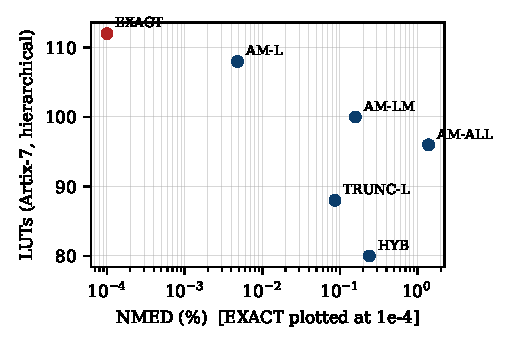
\includegraphics[width=0.65\textwidth]{fig_tradeoff.pdf}
\caption{LUT count versus NMED (EXACT plotted at $10^{-4}$ for the logarithmic axis).}
\label{fig:trade}
\end{figure}

\section{Image-Processing Results}
Table~\ref{tab:img} lists PSNR and SSIM for the three applications, and Figure~\ref{fig:img} shows the output images.

\begin{table}[ht]
\centering
\caption{Image quality compared with exact multiplication: PSNR (dB) / SSIM}
\label{tab:img}
\begin{tabular}{lccc}
\toprule
Design & Image multiplication & Gaussian smoothing & Image blending \\
\midrule
AM-L    & 64.81 / 0.9998 & identical ($\infty$ / 1.0000) & 60.93 / 0.9996 \\
AM-LM   & 51.99 / 0.9973 & 56.17 / 0.9988 & 49.38 / 0.9980 \\
AM-ALL  & 35.27 / 0.9851 & 34.98 / 0.9959 & 34.16 / 0.9951 \\
TRUNC-L & 55.70 / 0.9984 & 51.50 / 0.9976 & 51.99 / 0.9980 \\
\textbf{HYB} & 50.12 / 0.9960 & 49.71 / 0.9972 & 46.66 / 0.9975 \\
\bottomrule
\end{tabular}
\end{table}

\begin{figure}[ht]
\centering
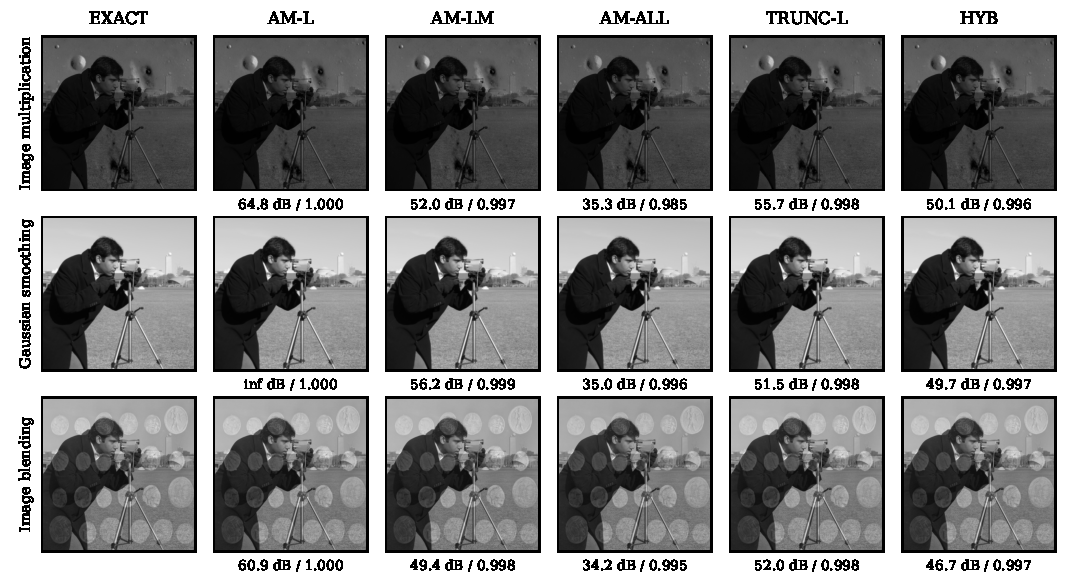
\includegraphics[width=\textwidth]{fig_images.pdf}
\caption{Output images of the three kernels for every multiplier (PSNR / SSIM against the exact output).}
\label{fig:img}
\end{figure}

\begin{itemize}
\item Every design except AM-ALL achieves PSNR above 46\,dB and SSIM of at least 0.996. At this level the outputs cannot be distinguished visually from the exact result (Figure~\ref{fig:img}).
\item AM-L produces a bit-identical Gaussian-smoothing output. An AM-L error needs a 2-bit field equal to 3 in the low nibble of both operands, and the low nibbles of the kernel weights (20, 32, 48) never contain one.
\item AM-ALL falls to about 34--35\,dB, consistent with its much larger worst-case error.
\item HYB keeps PSNR between 46.7 and 50.1\,dB while using the fewest LUTs.
\end{itemize}

\section{Basys-3 Demonstration Design}
The complete demonstration system, with all six multipliers, the debounced mode selection and the seven-segment driver, synthesises to 657 LUTs, 78 CARRY4 cells and 75 flip-flops in the Yosys flow, about 3.2\% of the 20{,}800 LUTs of the XC7A35T. Place-and-route, timing closure at 100\,MHz, power estimation and bitstream generation are performed in Vivado with the script in Appendix~\ref{app:fpga}.

\section{Limitations}
\begin{itemize}
\item Resource figures come from an open-source synthesis flow. Vivado implementation results (post-route LUTs, maximum frequency and power) should be added from the reports generated by the provided script; absolute LUT counts will differ from Yosys.
\item The error of all approximate designs is one-sided. A constant compensation term would reduce the mean error but has not been evaluated.
\item TRUNC-L and HYB return zero when both operands are below 16, which makes them unsuitable for kernels that multiply many small numbers.
\item The image applications were evaluated in software using the RTL product tables, not in a hardware image pipeline.
\end{itemize}

% =========================================================== CHAPTER 7
\chapter{Conclusion and Future Scope}

\section{Conclusion}
A parameterised family of six recursive 8$\times$8 unsigned multipliers was designed in Verilog HDL, verified exhaustively over all 65{,}536 input pairs, synthesised for the Xilinx 7-series (Artix-7) fabric used on the Basys-3 board, and evaluated in three image-processing applications. The main conclusions are:
\begin{enumerate}
\item The significance of the approximated partial product determines both the error and the saving. Approximating only $A_LB_L$ gives almost exact results (NMED 0.0048\%), while approximating all four partial products gives a worst-case error of 22\%.
\item On LUT-based FPGAs, removing the lowest partial product (TRUNC-L) saves more LUTs and gives lower mean error than applying the under-designed block to the middle and upper partial products.
\item The proposed hybrid design HYB saves 28.6\% of LUTs in the hierarchical flow (39.8\% in a flattened flow) with NMED 0.24\%, and keeps image PSNR between 46.7 and 50.1\,dB and SSIM of at least 0.996.
\end{enumerate}

\section{Future Scope}
\begin{itemize}
\item Run the provided Vivado script to obtain post-route utilisation, timing and power on the Basys-3 board, and measure power on hardware.
\item Add constant bias compensation to reduce the mean error of TRUNC-L and HYB.
\item Extend the design to signed operands and to 16$\times$16 multipliers.
\item Integrate HYB into a streaming convolution or neural-network accelerator on the FPGA and evaluate end-to-end accuracy.
\item Compare with Vivado's LogiCORE multiplier and with the DSP48E1 implementation for throughput and energy per operation.
\end{itemize}

% =========================================================== REFERENCES
\bibliographystyle{IEEEtran}
\bibliography{../paper/refs}

% =========================================================== APPENDICES
\appendix

\chapter{Verilog RTL Source Code}
\label{app:rtl}
The 2$\times$2, 4$\times$4 and 8$\times$8 modules are listed in Chapter~4 (Listings~\ref{lst:m2}--\ref{lst:m8}). The registered wrapper follows.
\lstinputlisting[language=VerilogX, caption={Registered wrapper (\texttt{rtl/mul8x8\_pipe.v})}]{../rtl/mul8x8_pipe.v}

\chapter{Testbenches}
\label{app:tb}
\lstinputlisting[language=VerilogX, caption={Exhaustive self-checking testbench (\texttt{tb/tb\_exhaustive.v})}]{../tb/tb_exhaustive.v}
\lstinputlisting[language=VerilogX, caption={Clocked waveform testbench (\texttt{tb/tb\_wave.v})}]{../tb/tb_wave.v}

\chapter{FPGA Implementation Files}
\label{app:fpga}
\lstinputlisting[language=VerilogX, caption={Basys-3 top level (\texttt{fpga/basys3\_top.v})}]{../fpga/basys3_top.v}
\lstinputlisting[language={}, caption={Basys-3 constraints (\texttt{fpga/basys3.xdc})}]{../fpga/basys3.xdc}
\lstinputlisting[language={}, caption={Vivado batch script (\texttt{fpga/vivado\_build.tcl})}]{../fpga/vivado_build.tcl}

\section*{Steps to program the Basys-3 board in Vivado (GUI)}
\begin{enumerate}
\item Create a new RTL project for part \texttt{xc7a35tcpg236-1} (Basys-3).
\item Add \texttt{rtl/mul2x2.v}, \texttt{rtl/mul4x4.v}, \texttt{rtl/mul8x8.v} and \texttt{fpga/basys3\_top.v} as design sources, and \texttt{fpga/basys3.xdc} as the constraint file. Check the pin assignments against the Digilent master XDC.
\item Set \texttt{basys3\_top} as the top module, then run Synthesis, Implementation and Generate Bitstream.
\item Open the Hardware Manager, connect to the board over USB and program the device.
\item Set operands on the switches, read the product on the LEDs, and press BTNU/BTND to change the multiplier mode. The seven-segment display shows the mode and the error.
\end{enumerate}

\chapter{Synthesis and Analysis Scripts}
\lstinputlisting[language=bash, caption={Yosys synthesis script (\texttt{synth/synth.sh})}]{../synth/synth.sh}
\lstinputlisting[language=bash, caption={One-command reproduction script (\texttt{run\_all.sh})}]{../run_all.sh}
\lstinputlisting[language=Python, caption={Analysis script (\texttt{analysis/analyze.py})}]{../analysis/analyze.py}

\end{document}
